\chapter{Implementation and testing}
Following the design, the implementation aimed to fulfill it and the requirements. Some changes were made to the implementation according to the feed back of the Causcumber team. Since Causcumber are built with python, this tool will also be built will python to reduce the chance of any potential problem happening. The tool will primary be a front end for Causcumber, and it will be built with Kivy, an open source python library mainly for develop user interface and application \cite{Reference20}. 

\section{Overview}
This project will utilize the Screen and ScreenManager function in Kivy. This design is due to many steps in testing with Causcumber require different syntax, to make this clearer for user, different syntax is assigned to different screen. With this, different screen will have different composition to reflect each syntax, extra functions are added to some screens to assist user in editing. This design also allows the development process be more efficient and concise. Since if there’s any new function required to be added, developer can simply create a new screen with new function and use ScreenManager to connect it to existing screen, and the new function can be organized into file(s) to keep the codes concise. Since Causcumber require several mandatory files to work, user will need to go through several steps before execute the test, below is the basic workflow of the tool:
\begin{figure}[H]
	\centering
	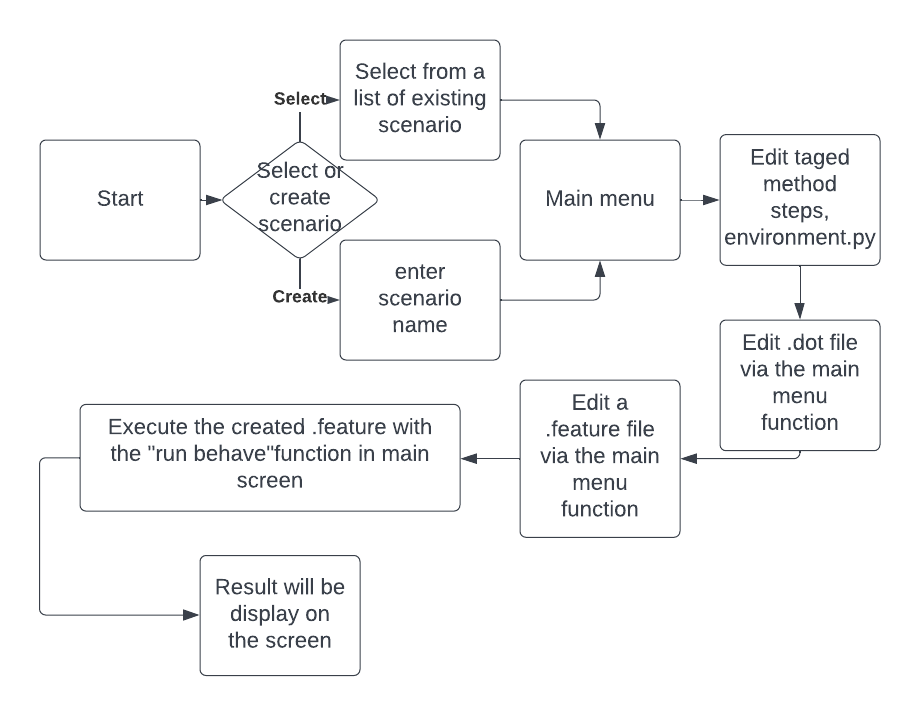
\includegraphics[width=10cm]{figures/workFlow.png}\\
	\caption{Basic workflow for testing a model.}
	\label{fig:figure9}
\end{figure}


\section{Create and select scenario}
In the beginning, Causcumber require user to create scenario directory, a scenario contains two mandatory sub-directories, \textsl{dags}, a directory contain causal graphs that defines the relations of parameter as \textsl{.dot} file. The second sub-directories is \textsl{features}, a directory where user can create \textsl{.feature} file that contain element for behave \cite{Reference21}. It also contain \textsl{environment.py} file, and a sub-directory \textsl{steps} that has scripts to implement step definitions for \textsl{.feature} file. The tool will allow user to create or select and existing scenario, upon create a new scenario, the tool will generate the basic files and sub-directory required for a scenario. Upon starting the system, the user will have two options, select, and create scenario.
\begin{figure}[H]
	\centering
	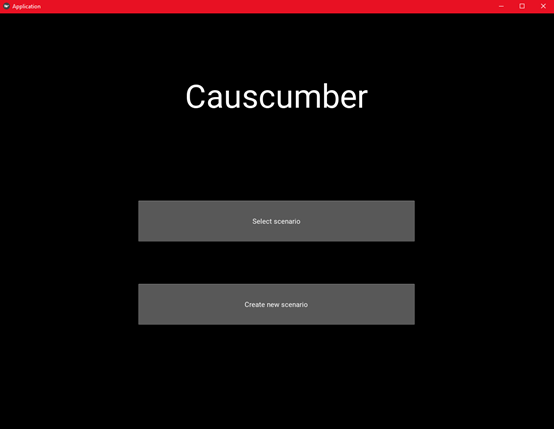
\includegraphics[width=10cm]{figures/startScreen.png}\\
	\caption{Start screen.}
	\label{fig:figure10}
\end{figure}
\noindent 
If user choose to select existing scenario, they will be presented with a list of existing scenarios to choose from. If user choose to create a new scenario, user will be prompt to enter the scenario name.
\begin{figure}[H]
	\centering
	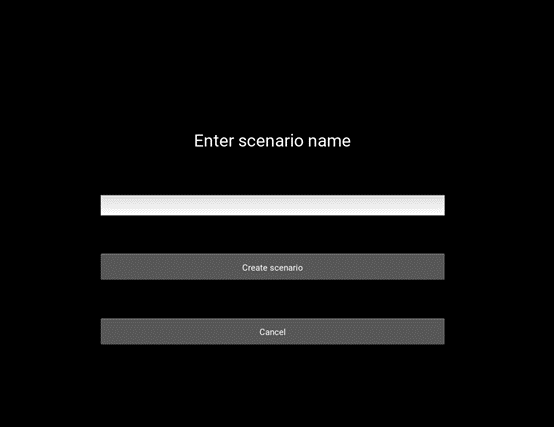
\includegraphics[width=10cm]{figures/createNewScenario.png}\\
	\caption{Create new scenario screen.}
	\label{fig:figure11}
\end{figure}
\noindent 
The tool will create files with custom file and method name based on the scenario name entered by the user.

\section{Main screen}
In the basic version of Causcumber, to execute test, user will need to use terminal and run the command “behave features/{feature filename}”. In the main screen, user can achieve this by simple use the “Select feature file” to chose the target \textsl{.feature} file, and “run behave” to execute the test. Then the result will be display on the screen in the result section, if the user has 95\% Confidence interval in the result they produce, the interval will recorded and plot it in the graph under the result section(see appendix A.1). But before this, user will need to go through some steps to setup the test.
\begin{figure}[H]
	\centering
	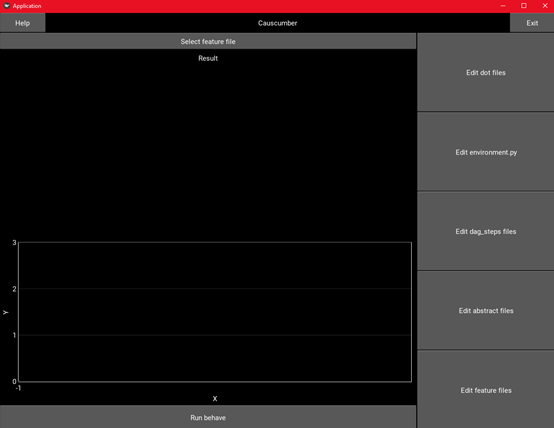
\includegraphics[width=10cm]{figures/mainScreen.png}\\
	\caption{Main screen.}
	\label{fig:figure12}
\end{figure}
\noindent 
The steps required is placed from top to bottom at the right of the screen as shown above, user will need to finish all the steps in order to test a model. A help section on top left is also provided to guide user if needed.


\section{Edit .dot file}
In the \textsl{.dot} file, user will first need to define the parameter clusters, typically there will be two clusters, one for input parameters and another for output parameters. After that user will need to define the relation between the parameters, this is done by using the syntax \textsl{ parameter1 -$>$ parameter2}. One useful feature for \textsl{.dot} file is combine with Graphviz, an open source graph visualization software, user can generate a graph that help visualize the relation and cluster. 
\begin{figure}[H]
	\centering
	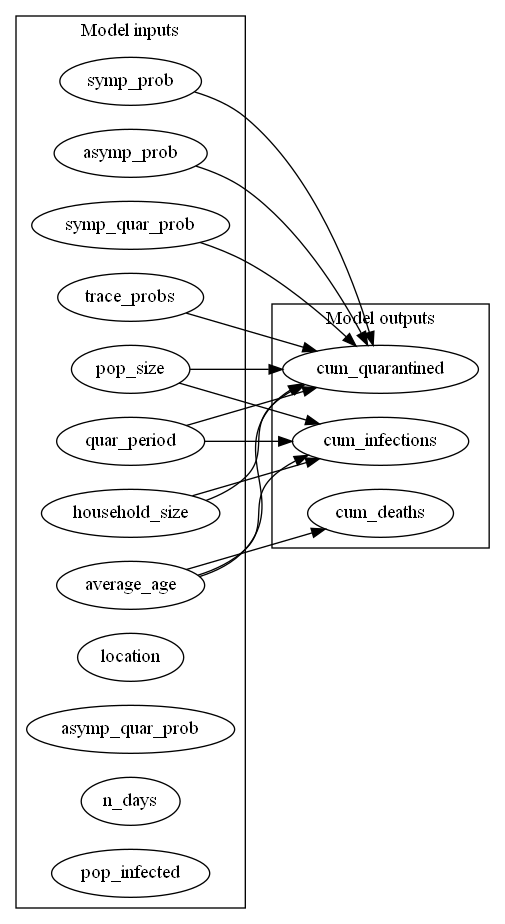
\includegraphics[width=10cm]{figures/dotExample.png}\\
	\caption{Graphviz example.}
	\label{fig:figure13}
\end{figure}
\noindent 
In the user interface, Graphviz is used to assist in the process. After click on the “Edit dot files” button in the menu, user will be brought to the screen for editing parameter clusters. 
\begin{figure}[H]
	\centering
	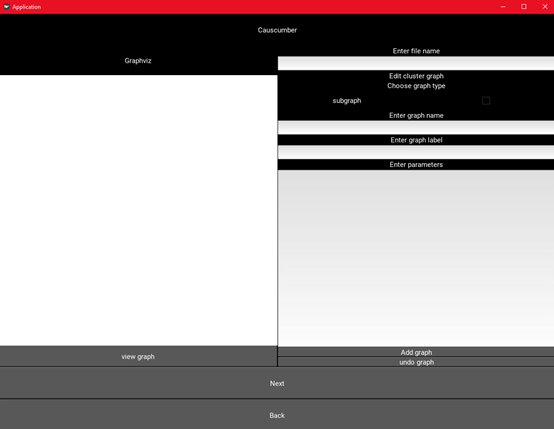
\includegraphics[width=10cm]{figures/editDot1Screen.png}\\
	\caption{Add parameter to .dot file.}
	\label{fig:figure14}
\end{figure}
\noindent 
At the right side, user will need to enter the filename, this can either be an existing file or a new file. Next user can change the syntax of the graph by tick or untick the subgraph checkbox, after user will need to enter the graph name and label. Then in the last section, enter parameters, user can enter the parameter for the graph.\\*\\*
After user input all the parameters, user can click next to go to the next step to edit relation of the parameters. Same as before, user should enter the filename, after that user need to click on the “Update parameter relation”, then the interface will display parameters entered in the previous step. By clicking the “select parameter”, a drop down menu will open for user to select a parameter, by select a parameter, that mean the selected parameter is related to the parameters ticked below (Include itself if ticked). When finish editing relations, user can click the “add graph” button to input the graph. The result of the graph will be display at the left side of the screen to assist the user. 
\begin{figure}[H]
	\centering
	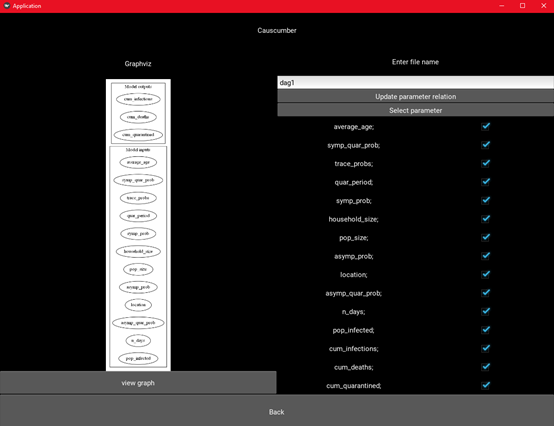
\includegraphics[width=10cm]{figures/editDot2Screen.png}\\
	\caption{Edit parameter relation.}
	\label{fig:figure15}
\end{figure}

\section{Setup background files}
Next, there are three background files require to setup. First in \textsl{environment.py}, user need to edit a \textsl{run\_[Model name]} method, the purpose of this file is to execute the testing model, user will need to modify it to able to run the model and return the result data. Second, is in \textsl{dag\_steps.py}, there are two parts require to be edit, custom distributions and metavariables. \\*\\*
For custom distributions, user is requiring to define class for distributions so that Causcumber can picks it up. The reason for why this needed is because default distributions in Causcumber uses SciPy, an open-source software for mathematics, science, and engineering \cite{Reference22}, to generate valid parameters values between 0 and 1, but not all the parameters are numerical. Custom distributions are for these types of parameters, for example \textsl{location} in covasim, custom distributions should generate strings from a given set.\\*\\*
For metavariables, user can define metavariables in the Background. Metavariables, or metasyntactic variable in computer science is a placeholder name that has no meaning and will be substituted \cite{Reference23}. User can use this to modify data in data sets.\\*\\*
The third file is \textsl{abstract.py}, in this file user can define custom constrains for parameter value. This limits the distributions for test data generation. For all three files, it requires users to manually define it since different models may work differently and require different codes, use uniform generated codes may cause problem. In the main screen, buttons are provided to help user open these file, by clicking those button, the files will be open with default editor set by the user.

\section{Edit .feature files}
Finally, user can start edit the feature file. In feature file, user will need to define background, list edges, scenario outline and scenario. In background, user will need to define the parameters and the distribution, user can also define metavariables if needed. Then user will need to define variables are recorded at the end, last user can also define extra conditions for the scenario with \textsl{And} syntax in Cucumber. \\*\\*
In the next part, user will need the list the edges of models, this part allow Causcumber to focus on relations of parameters in model define by the user. Next is \textsl{Scenario outline}, in this part user can define changes in parameter and the expected outcome, this require user to provide \textsl{Example}. Finally is \textsl{Scenario}, this is mostly same as \textsl{Scenario outline} but without  \textsl{Example}.\\*\\*
All the parts mentioned above require user to formatted in a certain syntax, with the interface, the syntax is incorporated into the format of the interface’s design. Starting with background, user need to edit the feature file’s name, then user can start setting the parameters, parameters’ type and parameters’ value. Next user can add meta variables, this part isn’t necessary for feature file, and can be left empty. Next is the recorded variables, this part is similar to the meta variables but will generate different syntax upon create feature file. Last is the for user to add extra condition to the background if needed. This part is structured very similar to the \textsl{.feature} file’s syntax, but with some modification to make those syntax even more plain text.
\begin{figure}[H]
	\centering
	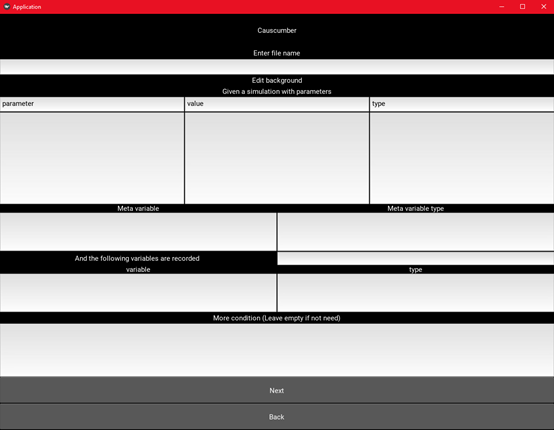
\includegraphics[width=10cm]{figures/editFeature1Screen.png}\\
	\caption{Edit first section of .feature file.}
	\label{fig:figure16}
\end{figure}
\noindent 
Next part is to define the edges, this part is mostly identical to the edit \textsl{.dot} function to keep the consistence of the system, the only new addition is a new option allow user to add new edges. This new function is added due to the potential need for user to add extra edges, user can choose to not add new edges if there’s no need for that.\\*\\*
After this is scenario outline and scenario, both are also structured like background, where parts of the sentence that require user to edit being left blank. In scenario outline, user will need to define “example”, which is how parameters will change when another parameter is changed in some way. The syntax for example is a table like structure, this is simulated in the interface where user can use the add column and add row to edit the example. 
\begin{figure}[H]
	\centering
	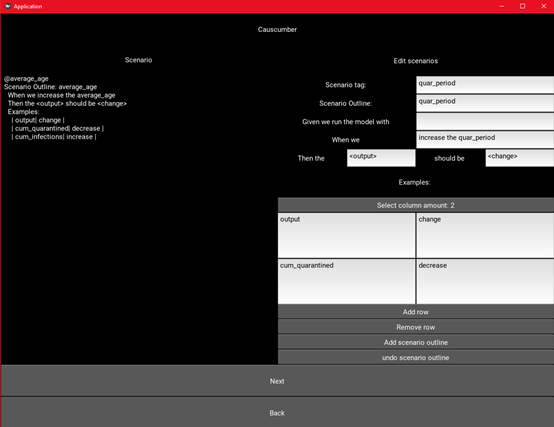
\includegraphics[width=10cm]{figures/editFeature2Screen.png}\\
	\caption{Edit scenario outline section of .feature file.}
	\label{fig:figure17}
\end{figure}
\noindent 
In scenario, instead of example, it uses “Then” and “And” structure in Cucumber to represent the expected result. The structure is similar to the previous page but with example replaced with the option to add “And”. The user will need to have at least one basic expected result, and if the user wishes to add more expected result, user can use “add And” option to add more. 
\begin{figure}[H]
	\centering
	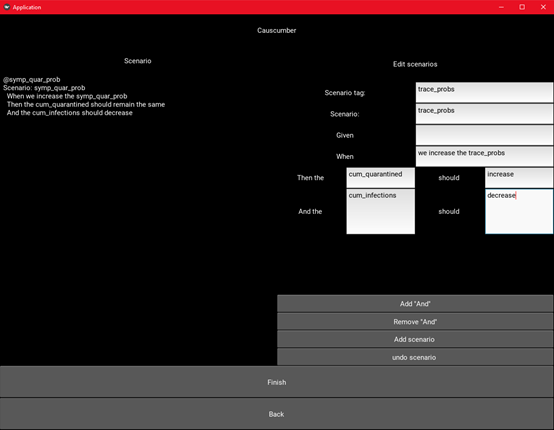
\includegraphics[width=10cm]{figures/editFeature3Screen.png}\\
	\caption{Edit scenario section of .feature file.}
	\label{fig:figure18}
\end{figure}
\noindent 
When done, user can just click “Finish” button to return to main menu, then select and run the feature file created.








